En este capítulo, se observan las diferentes pantallas que responden a las consultas realizadas a la MIB de Linux y de Windows y que de igual manera, muestra el segundo punto de la práctica que se refiere a la utilización del comando snmpget y algunos otros.
\section{Cuestionario}
\begin{enumerate}
\cfinput{Cuestionario/preguntasMarcela}
\cfinput{Cuestionario/preguntasRosa}
\cfinput{Cuestionario/preguntasSamuel}


\item ¿El agente ha recibido mensajes TCP? ¿Cuántos?\\
\textbf{Comando: snmpget (figura \ref{image:tcpget})}
\FloatBarrier
\begin{figure}[htbp!]
		\centering
	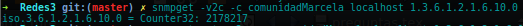
\includegraphics[width=.9 \textwidth]{images/tcpget}
		\caption{Número de mensajes TCP recibidos en Linux con comando snmpget.}		\label{image:tcpget}
\end{figure}
\FloatBarrier

\textbf{Comando: snmpgetnext (figura \ref{image:tcpnext})}
\FloatBarrier
\begin{figure}[htbp!]
		\centering
	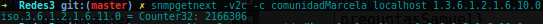
\includegraphics[width=.9 \textwidth]{images/tcpnext}
		\caption{Número de mensajes TCP recibidos en Linux con comando snmpgetnext.}		\label{image:tcpnext}
\end{figure}
\FloatBarrier

\textbf{Comando: snmpwalk (figura \ref{image:tcpwalk})}
\FloatBarrier
\begin{figure}[htbp!]
		\centering
	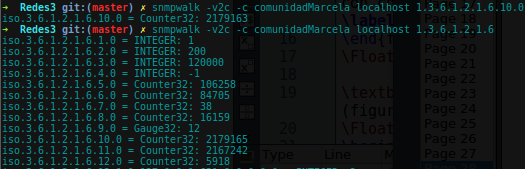
\includegraphics[width=.9 \textwidth]{images/tcpwalk}
		\caption{Número de mensajes TCP recibidos en Linux con comando snmpwalk.}		\label{image:tcpwalk}
\end{figure}
\FloatBarrier
\item ¿Cuántos mensajes EGP ha recibido el agente?

\item Indica el Sistema Operativo que maneja el agente.
\item Modifica el estatus administrativo (a down) de la interfaz que ha recibido más octetos.
\item Genera una alerta para avisar cuando se reinicie el agente.
\item Dibuja la MIB del agente.

Observamos en la figura \ref{image:dibujoMib}, la ejecución del comando \textbf{snmpwalk} al OID \textbf{1.3.6.1.2.1} correspondiente al objeto \textbf{mib-2}.
\FloatBarrier
\begin{figure}[htbp!]
		\centering
	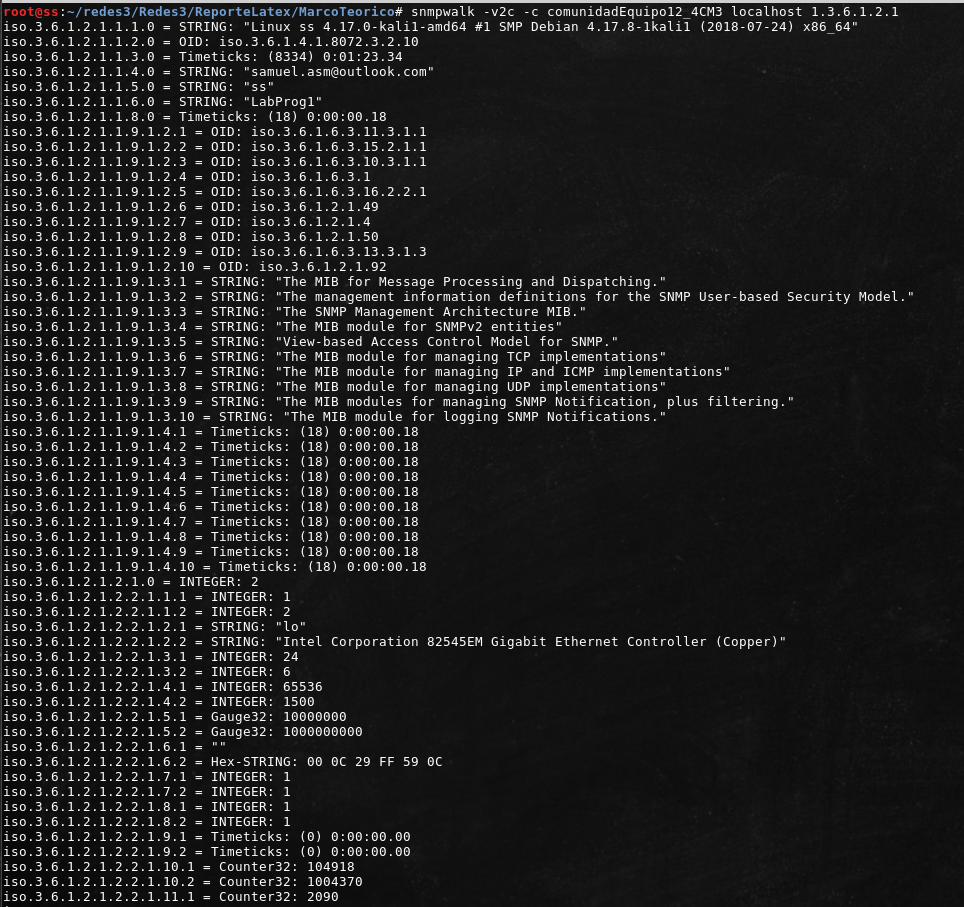
\includegraphics[width=.9 \textwidth]{images/dibujoMib}
		\caption{Dibujo de la MiB.}
\label{image:dibujoMib}
\end{figure}
\FloatBarrier
\end{enumerate}